\section{静电场中的导体}
\subsection{静电平衡}
将不带电的金属导体置于电场中，由静电感应现象在表面产生感应电荷，感应电荷不断积累，产生附加电场，最终达到导体内部电场强度处处为零，导体中没有任何电荷作定向运动，此状态称为\textbf{静电平衡}状态.需要注意的是该状态是没有电荷作定向运动而非没有电荷作运动，因为存在分子热运动.建立静电平衡的过程如图\ref{pic:7-6-1}所示.
\begin{figure}[hb]
    \begin{center}
        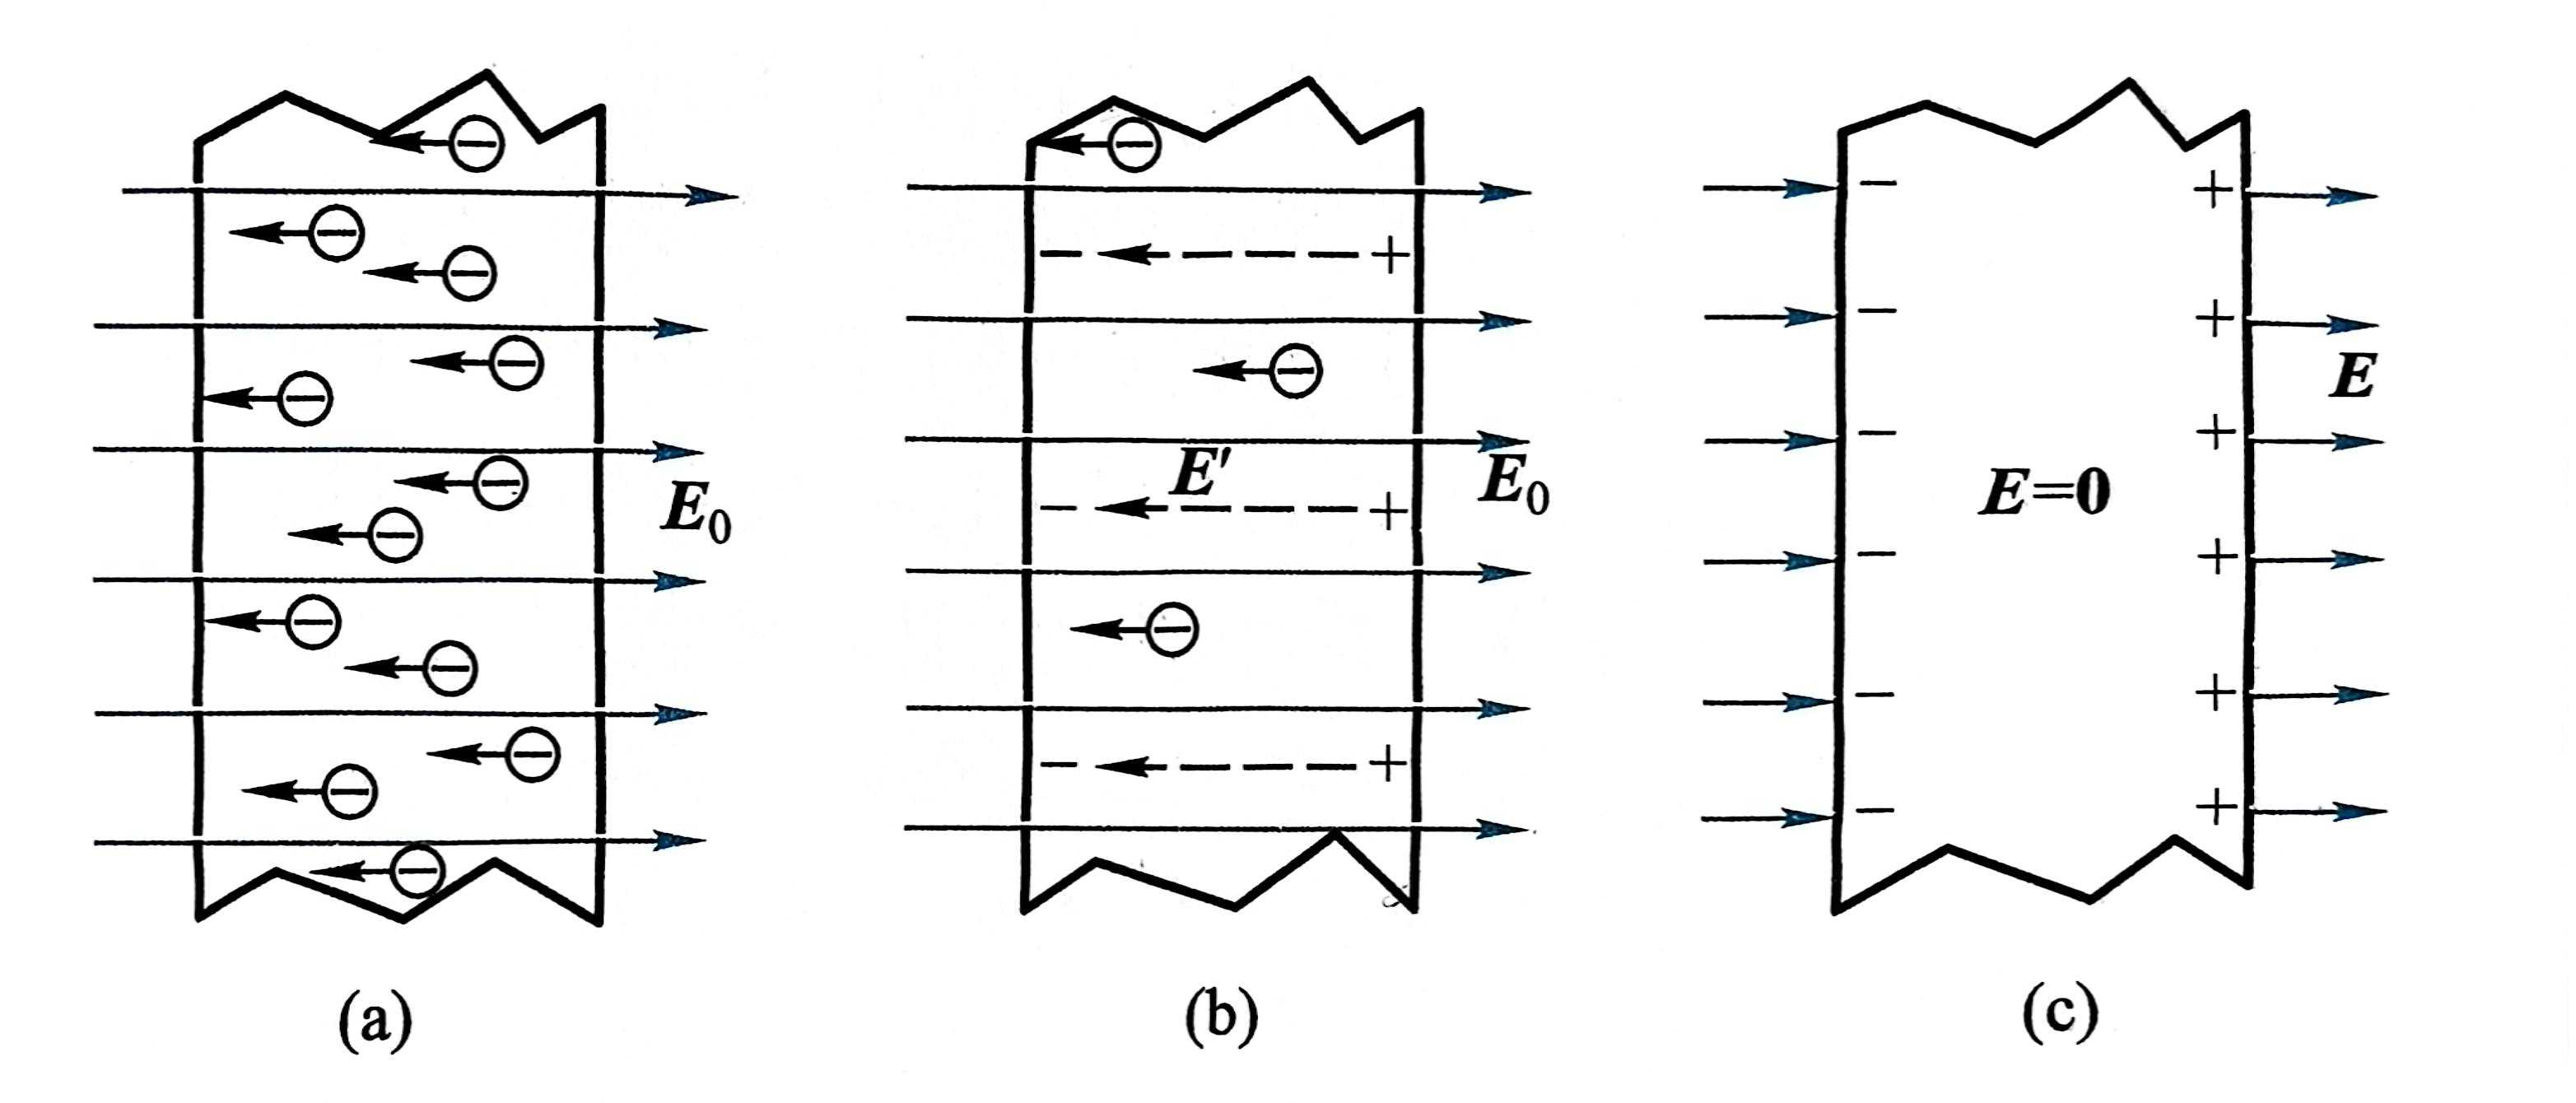
\includegraphics[width=0.6\textwidth]{images/7-6-1.jpg}
        \caption{静电感应过程}
        \label{pic:7-6-1}
    \end{center}
\end{figure}

根据导体静电平衡的条件，如图\ref{pic:7-6-2}所示，我们有以下推论：
\begin{enumerate}
    \item 导体是等势体，其表面是等势面.
    \item 导体表面的电场强度垂直于导体表面.
\end{enumerate}

\begin{figure}[hb]
    \begin{center}
        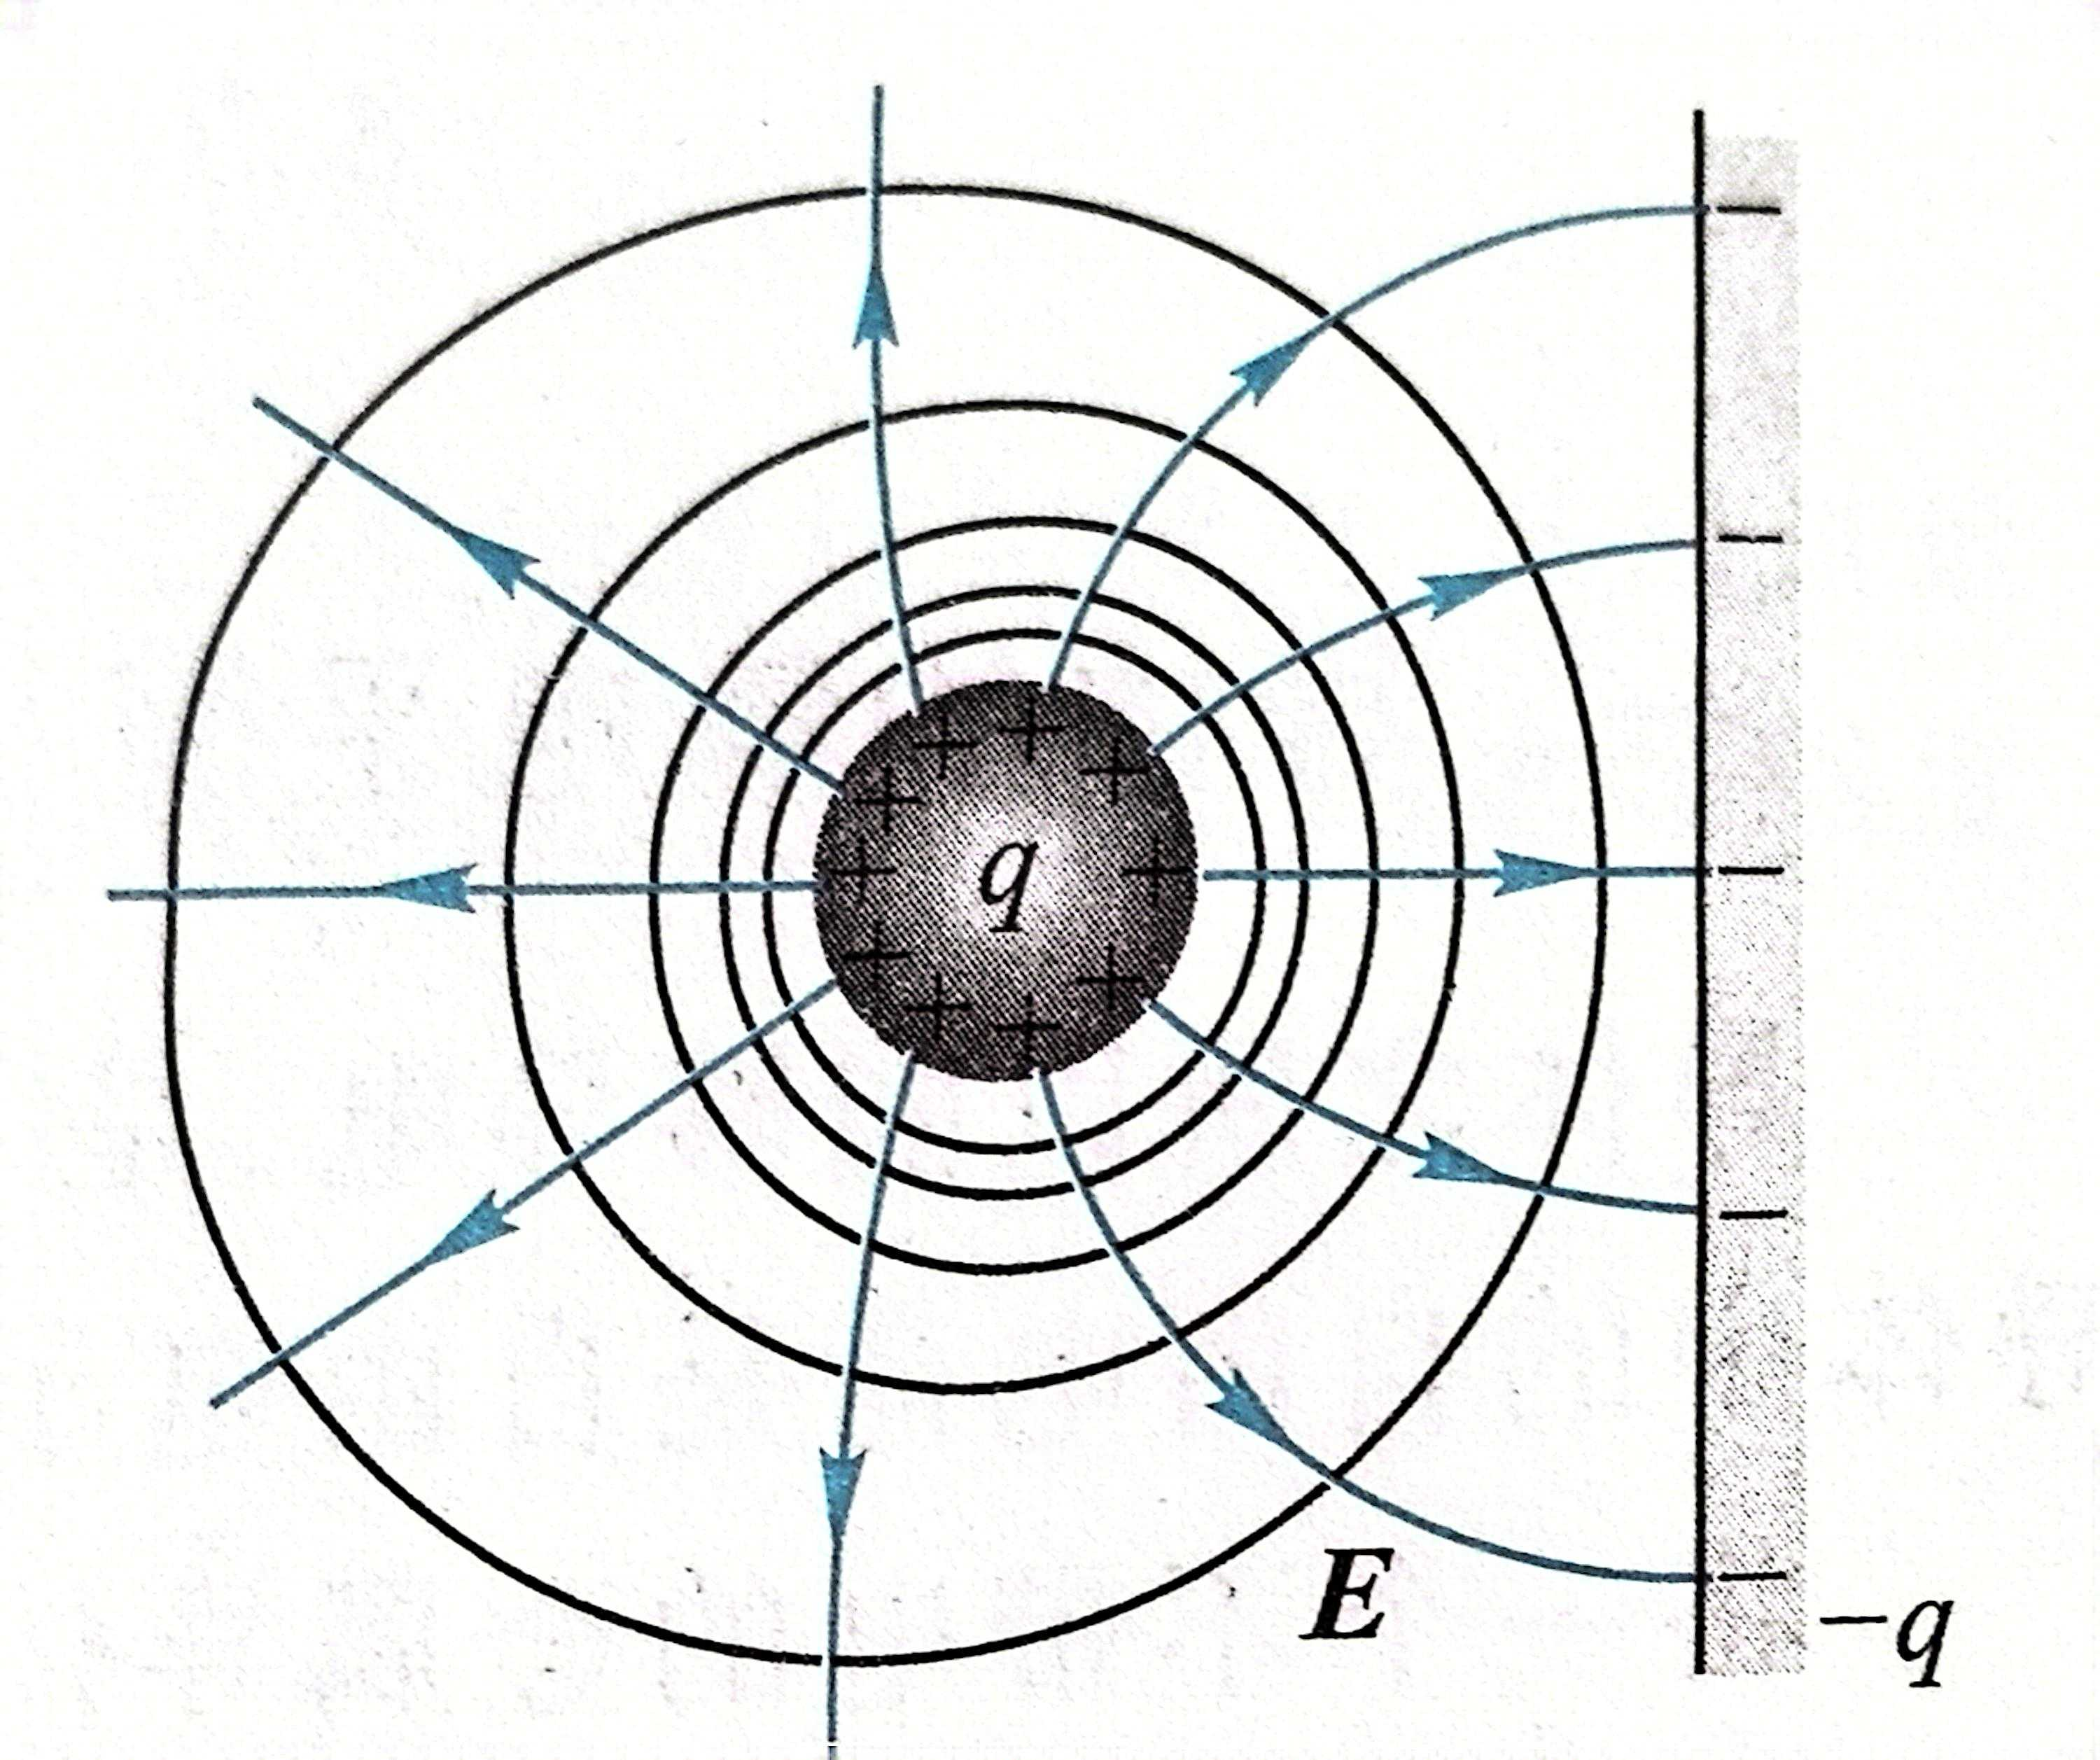
\includegraphics[width=0.4\textwidth]{images/7-6-2.jpg}
        \caption{导体附近电场/等势面分布}
        \label{pic:7-6-2}
    \end{center}
\end{figure}

\subsection{静电平衡时导体上的电荷分布}
根据高斯定理，当带点导体处于静电平衡状态时，电荷只能分布于导体的表面上（仅有感应电荷）.如果导体有空腔，空腔内有电荷时，导体内表面带有与电荷电量相等电性相反的感应电荷；空腔内没有电荷时，导体只有外表面带有感应电荷.


如图\ref{pic:7-6-3}方式取高斯面，由高斯定理，有带电导体表面附近的电场强度公式
\[
\bm{E}=\dfrac{\sigma}{\epsilon_0}\bm{e}_n
\]
\begin{figure}[h]
    \begin{center}
        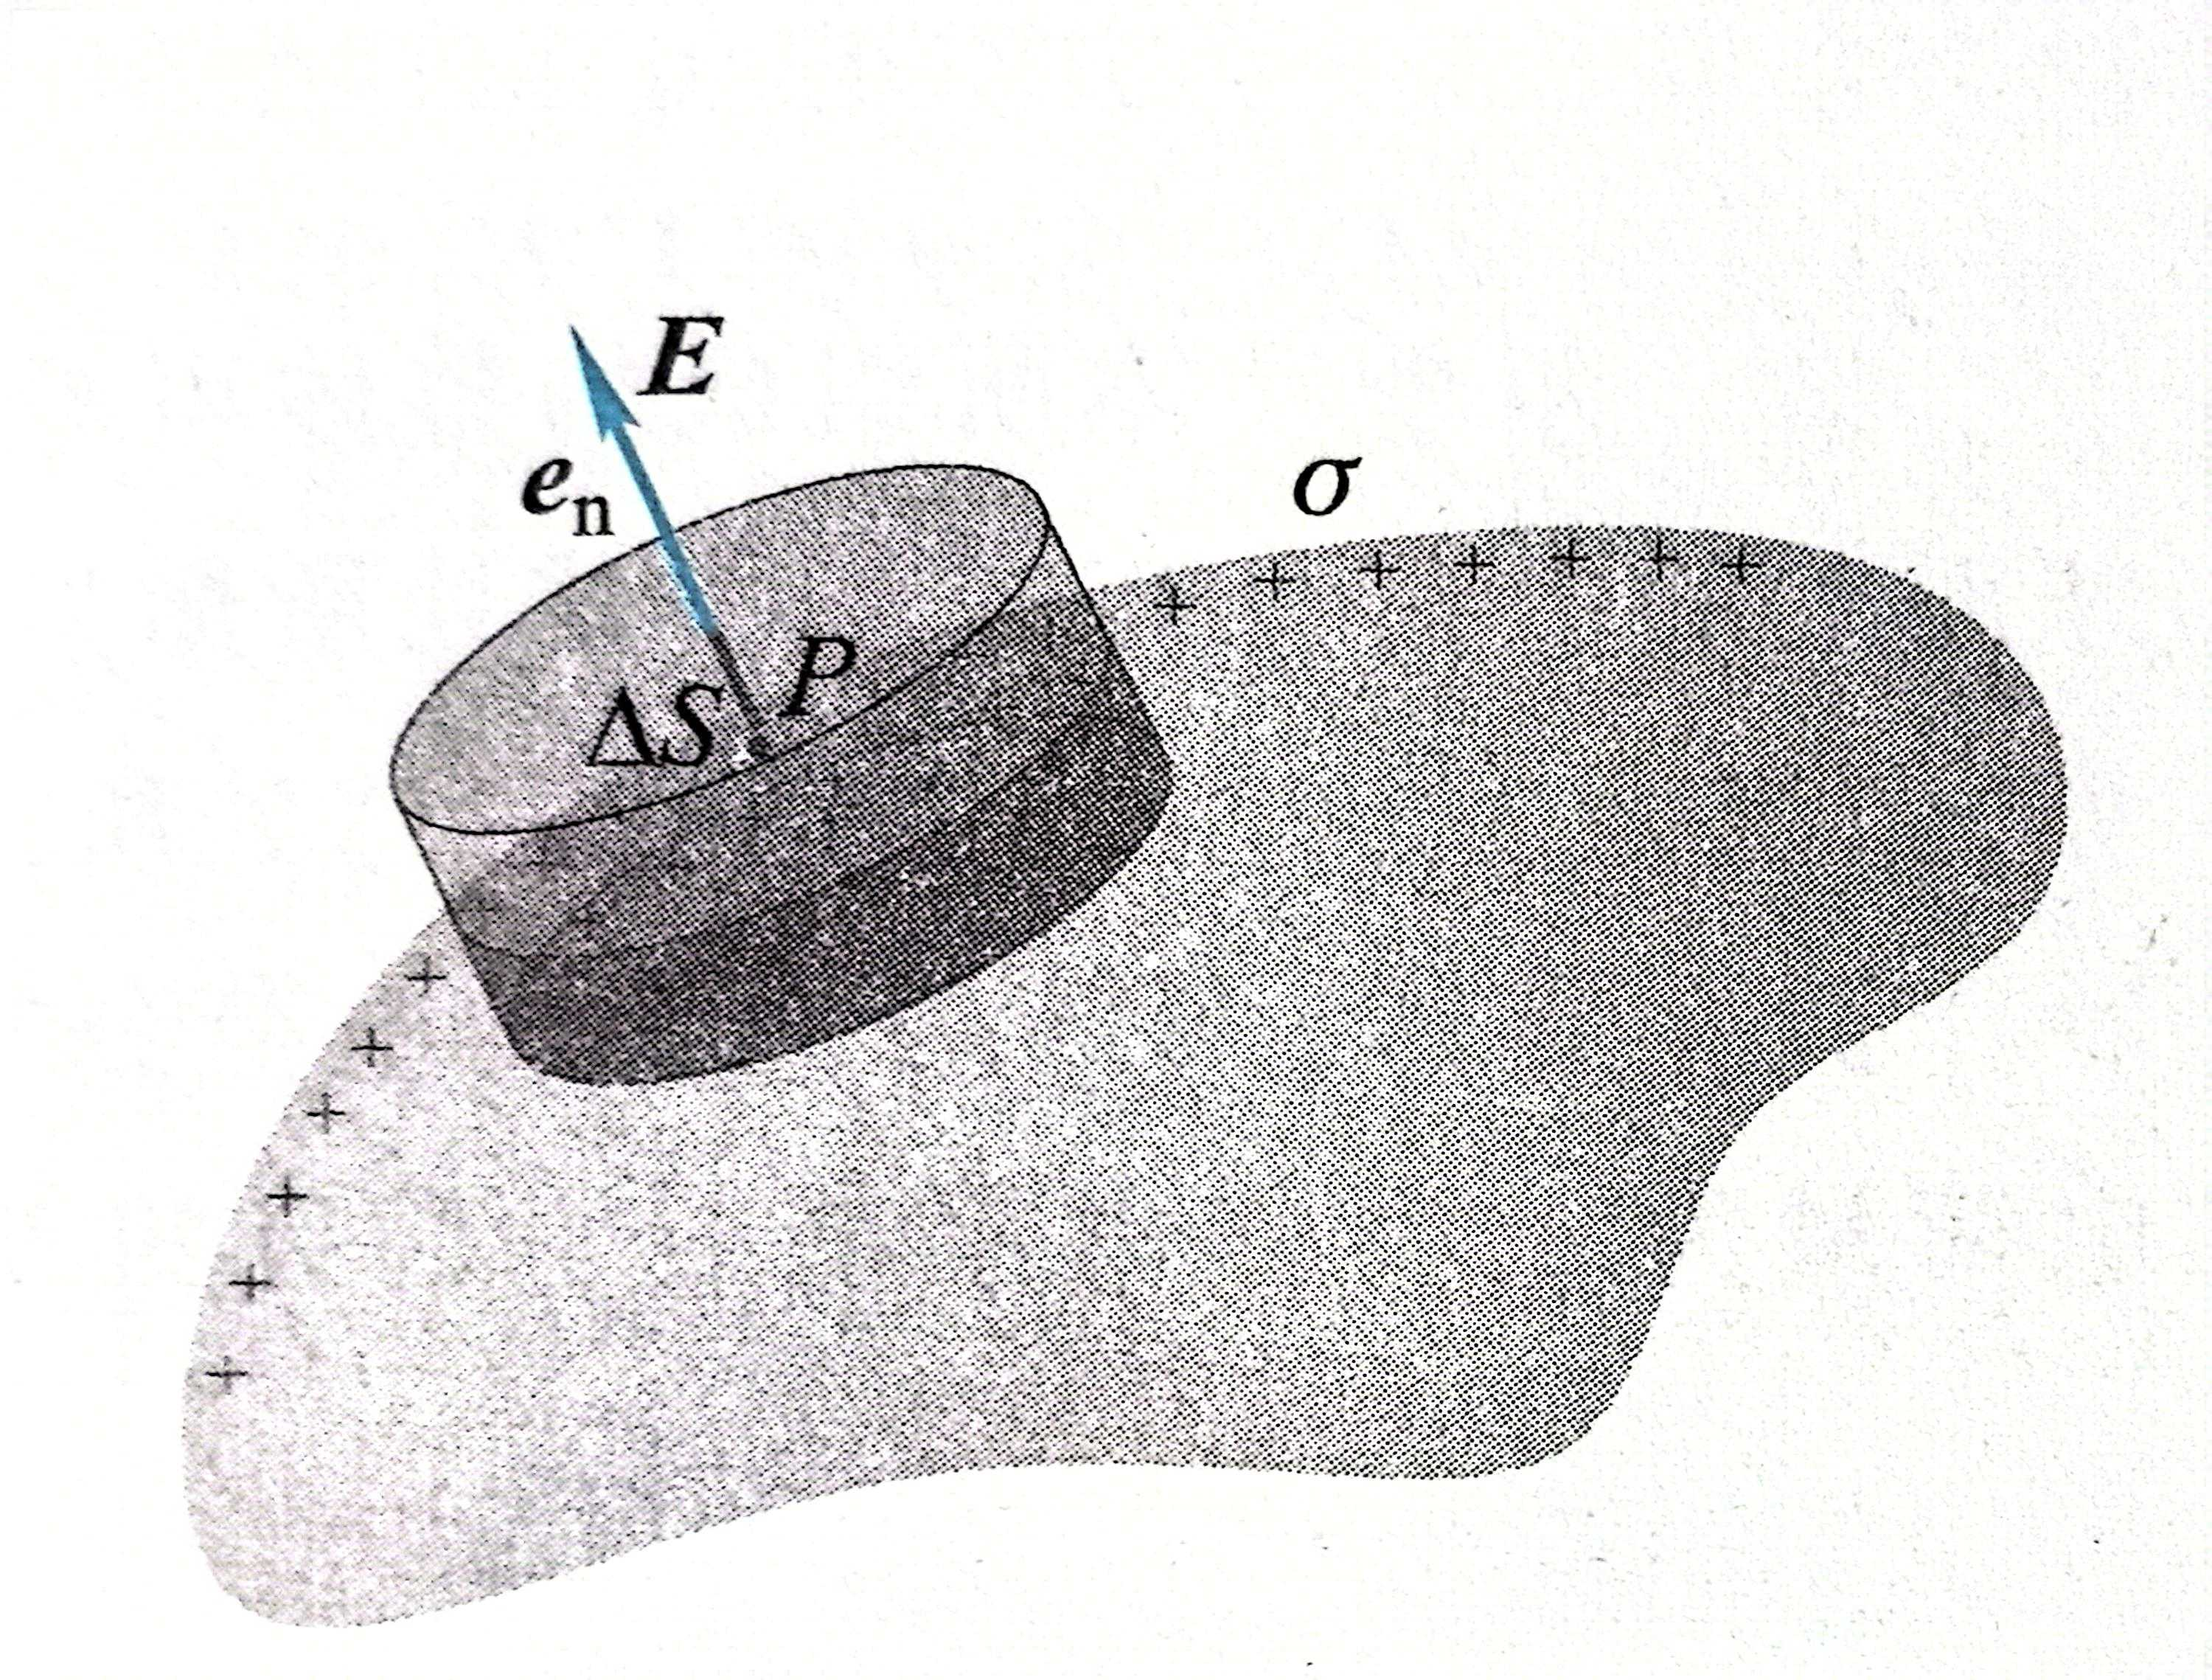
\includegraphics[width=0.4\textwidth]{images/7-6-3.jpg}
        \caption{导体表面附近的高斯面取法}
        \label{pic:7-6-3}
    \end{center}
\end{figure}
\begin{attention}{ }{7.6.1} % 添加标签参数
不要将该公式与无限大均匀带电平面产生的电场强度混淆！事实上，这两个公式说明的是一个问题，只不过电荷面密度代表的含义有所差别.
\end{attention}

对于孤立的带电导体，感应电荷在其表面的分布由其表面曲率确定.曲率越大，电荷分布越密集，此处曲率的符号表征“大小”.只有孤立导体球表面电荷分布均匀.

\subsection{静电屏蔽}
在静电平衡的条件下，导体空腔外的带电体不会影响腔内的电场分布；接地的空腔导体腔内电荷不会影响腔外的电场分布.这就是\textbf{静电屏蔽}效应.